\documentclass[letterpaper,12pt]{article}

\usepackage{threeparttable}
\usepackage{geometry}
\geometry{letterpaper,tmargin=1in,bmargin=1in,lmargin=1.25in,rmargin=1.25in}
\usepackage[format=hang,font=normalsize,labelfont=bf]{caption}
\usepackage{amsmath}
\usepackage{multirow}
\usepackage{array}
\usepackage{delarray}
\usepackage{amssymb}
\usepackage{amsthm}
\usepackage{lscape}
\usepackage{natbib}
\usepackage{setspace}
\usepackage{float,color}
\usepackage[pdftex]{graphicx}
\usepackage{listings}
\lstset{basicstyle=\footnotesize\ttfamily, language=Python, showstringspaces=false}

\lstset{frame=single,
  language=Python,
  showstringspaces=false,
  columns=flexible,
  basicstyle={\small\ttfamily},
  numbers=none,
  breaklines=true,
  breakatwhitespace=true
  tabsize=3
}

\usepackage{pdfsync}
\usepackage{verbatim}
\usepackage{placeins}
\usepackage{geometry}
\usepackage{pdflscape}
\synctex=1
\usepackage{hyperref}
\hypersetup{colorlinks,linkcolor=red,urlcolor=blue,citecolor=red}
\usepackage{bm}


\theoremstyle{definition}
\newtheorem{theorem}{Theorem}
\newtheorem{acknowledgement}[theorem]{Acknowledgement}
\newtheorem{algorithm}[theorem]{Algorithm}
\newtheorem{axiom}[theorem]{Axiom}
\newtheorem{case}[theorem]{Case}
\newtheorem{claim}[theorem]{Claim}
\newtheorem{conclusion}[theorem]{Conclusion}
\newtheorem{condition}[theorem]{Condition}
\newtheorem{conjecture}[theorem]{Conjecture}
\newtheorem{corollary}[theorem]{Corollary}
\newtheorem{criterion}[theorem]{Criterion}
\newtheorem{definition}{Definition} % Number definitions on their own
\newtheorem{derivation}{Derivation} % Number derivations on their own
\newtheorem{example}[theorem]{Example}
\newtheorem{exercise}[theorem]{Exercise}
\newtheorem{lemma}[theorem]{Lemma}
\newtheorem{notation}[theorem]{Notation}
\newtheorem{problem}[theorem]{Problem}
\newtheorem{proposition}{Proposition} % Number propositions on their own
\newtheorem{remark}[theorem]{Remark}
\newtheorem{solution}[theorem]{Solution}
\newtheorem{summary}[theorem]{Summary}
\bibliographystyle{aer}
\newcommand\ve{\varepsilon}
%\renewcommand\theenumi{\roman{enumi}}
\newcommand\norm[1]{\left\lVert#1\right\rVert}

\begin{document}

\title{Demographic transition forecasting notes}
\date{version (20.02.a)}
\author{Richard W. Evans}
\maketitle

\pagenumbering{arabic}


This document provides the theory and computational tools to forecast the population by age $\omega_{s,t}$ given current trends in fertility rates, mortality rates, and immigration rates.


\section{Demographics Theory}\label{SecTheory}

  Define $\omega_{s,t}$ as the number of age-$s$ individuals alive at time $t$. A measure $\omega_{1,t}$ of individuals is born in each period $t$ and live for up to $E+S$ periods, with $S\geq 3$. Individuals are termed ``youth'', and do not participate in market activity during ages $1\leq s\leq E$. Individuals enter the workforce and economy in period $E+1$ and remain in the workforce until they unexpectedly die or live until age $s=E+S$. We model the population with individuals age $s\leq E$ outside of the workforce and economy in order most closely match the empirical population dynamics.

  The population of individuals of each age in each period $\omega_{s,t}$ evolves according to the following function,
  \begin{equation}\label{EqPopLawofmotion}
    \begin{split}
      \omega_{1,t+1} &= (1 - \rho_{0,t})\sum_{s=1}^{E+S} f_{s,t}\omega_{s,t} + i_{1,t+1}\omega_{1,t}\quad\forall t \\
      \omega_{s+1,t+1} &= (1 - \rho_{s,t})\omega_{s,t} + i_{s+1,t+1}\omega_{s+1,t}\quad\forall t\quad\text{and}\quad 1\leq s \leq E+S-1
    \end{split}
  \end{equation}
  where $f_{s,t}\geq 0$ is an age- and period-specific fertility rate, $i_{s,t}$ is an age- and period-specific net immigration rate, $\rho_{s,t}$ is an age- and period-specific mortality hazard rate, and $\rho_{0,t}$ is a period-specific infant mortality rate.\footnote{The parameters $\rho_{s,t}$ represent the probability that an individual of age $s$ dies before age $s+1$.} The total population in the economy $N_t$ at any period is simply the sum of households in the economy, the population growth rate in any period $t$ from the previous period $t-1$ is $g_{n,t}$, $\tilde{N}_t$ is the working age population, and $\tilde{g}_{n,t}$ is the working age population growth rate in any period $t$ from the previous period $t-1$.
  \begin{equation}\label{EqPopN}
    N_t\equiv\sum_{s=1}^{E+S} \omega_{s,t} \quad\forall t
  \end{equation}
  \begin{equation}\label{EqPopGrowth}
    g_{n,t+1} \equiv \frac{N_{t+1}}{N_t} - 1 \quad\forall t
  \end{equation}
  \begin{equation}\label{EqPopNtil}
    \tilde{N}_t\equiv\sum_{s=E+1}^{E+S} \omega_{s,t} \quad\forall t
  \end{equation}
  \begin{equation}\label{EqPopGrowthTil}
    \tilde{g}_{n,t+1} \equiv \frac{\tilde{N}_{t+1}}{\tilde{N}_t} - 1 \quad\forall t
  \end{equation}

  The following subsections describe how to estimate, calibrate, and forecast the fertility rates $\{f_{s,t}\}_{s=1,t=T_{beg}}^{E+S,T_{end}}$, mortality rates $\{\rho_{s,t}\}_{s=0,t=T_{beg}}^{E+S,T_{end}}$, and immigration rates $\{i_{s,t}\}_{s=1,t=T_{beg}}^{E+S,T_{end}}$ in order to forecast the population dynamics $\{\omega_{s,t}\}_{s=1,t=0}^{E+S,T_{end}}$.


  \subsection{Fertility rates}\label{SecFert}

    Define the fertility rate as $f_{s,t}$ which signifies the percent of age-$s$ individuals that have children in year $t$. This fertility rate must account for both male and female population. The data below are U.S. fertility rates by age from \citet[Table 3, p. 18]{MartinEtAl:2015} National Vital Statistics Report, which is final fertility rate data for 2013. Figure \ref{FigFertRates} shows the fertility-rate data and the estimated average fertility rates for $E+S=100$.

    \begin{figure}[htbp]\centering \captionsetup{width=4.0in}
      \caption{\label{FigFertRates}\textbf{U.S. 2013 fertility rates by age ($f_{s,t=2013}$)}}
      \fbox{\resizebox{4.0in}{3.0in}{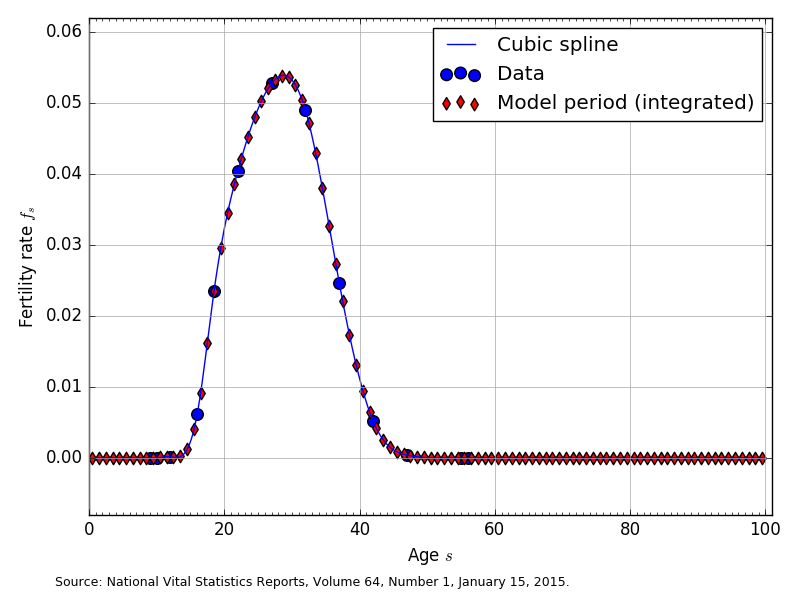
\includegraphics{./images/fert_rates.png}}}
    \end{figure}

    The large blue circles are the 2013 U.S. fertility rate data from \citet{MartinEtAl:2015}. These are 9 fertility rates $[0.3, 12.3, 47.1, 80.7, 105.5, 98.0, 49.3, 10.4, 0.8]$ that correspond to the midpoint ages of the following age (in years) bins $[10-14, 15-17, 18-19, 20-24, 25-29, 30-34, 35-39, 40-44, 45-49]$. In order to get our cubic spline interpolating function to fit better at the endpoints we added to fertility rates of zero to ages 9 and 10, and we added two fertility rates of zero to ages 55 and 56. The blue line in Figure \ref{FigFertRates} shows the cubic spline interpolated function of the data.

    The red diamonds in Figure \ref{FigFertRates} are the average fertility rate in age bins spanning households born at the beginning of period 1 (time = 0) and dying at the end of their 100th year. Let the total number of model years that a household lives be $E+S\leq 100$. Then the span from the beginning of period 1 (the beginning of year 0) to the end of period 100 (the end of year 99) is divided up into $E+S$ bins of equal length. We calculate the average fertility rate in each of the $E+S$ model-period bins as the average population-weighted fertility rate in that span. The red diamonds in Figure \ref{FigFertRates} are the average fertility rates displayed at the midpoint in each of the $E+S$ model-period bins.


  \subsection{Mortality rates}\label{SecMort}

    The mortality rates in this demographic model $\rho_{s,t}$ represent a one-period hazard rate and represent the probability of dying within one year, given that an individual is alive at the beginning of age $s$ in period $t$. The infant mortality rate of $\rho_{0,t=2015}=0.00587$ comes from the 2015 U.S. CIA World Factbook. The data in Figure \ref{FigMortRates} for U.S. mortality rates by age come from the Actuarial Life Tables of the U.S. Social Security Administration \citep[see][]{SocSec:2015}, from which the most recent mortality rate data is for 2011. Figure \ref{FigMortRates} shows the mortality rate data and the corresponding model-period mortality rates for $E+S=100$.

    \begin{figure}[htbp]\centering \captionsetup{width=4.0in}
      \caption{\label{FigMortRates}\textbf{U.S. 2011 mortality rates by age ($\rho_{s,t=2011}$)}}
      \fbox{\resizebox{4.0in}{3.0in}{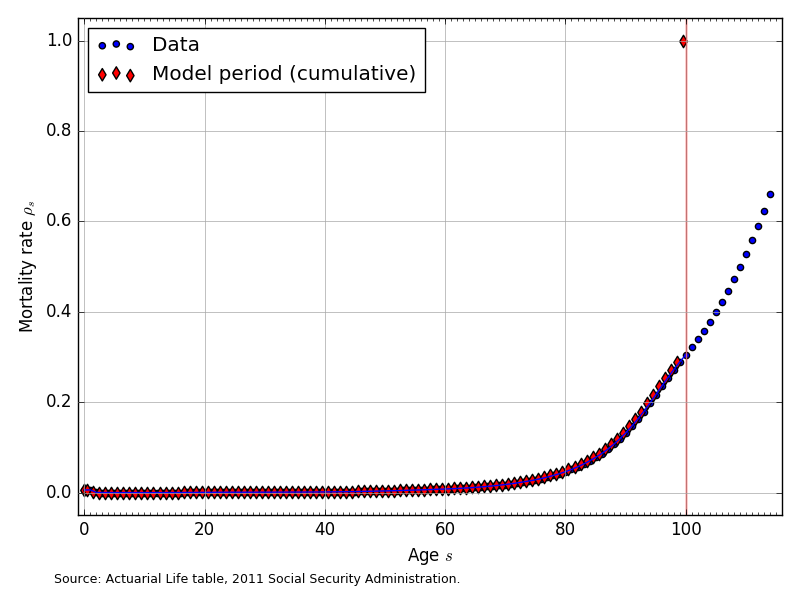
\includegraphics{./images/mort_rates.png}}}
    \end{figure}

    The mortality rates in Figure \ref{FigMortRates} are a population-weighted average of the male and female mortality rates reported in \citet{SocSec:2015}. Figure \ref{FigMortRates} also shows that the data provide mortality rates for ages up to 111-years-old. We truncate the maximum age in years in our model to 100-years old. In addition, we constrain the mortality rate to be 1.0 or 100 percent at the maximum age of 100.


  \subsection{Immigration rates}\label{SecImmig}

    Because of the difficulty in getting accurate immigration rate data by age, we estimate the immigration rates by age and period $i_{s,t}$ as the residual that reconciles the current-period population distribution with next period's population distribution given fertility rates $f_{s,t}$ and mortality rates $\rho_{s,t}$. Solving equations \eqref{EqPopLawofmotion} for the immigration rates $i_{s,t}$ gives the following characterization of the immigration rates in given population levels in any two consecutive periods $\omega_{s,t}$ and $\omega_{s,t+1}$ and the fertility rates $f_{s,t}$ and mortality rates $\rho_{s,t}$.

    \begin{equation}\label{EqPopImmRates}
      \begin{split}
        i_{1,t+1} &= \frac{\omega_{1,t+1} - (1 - \rho_{0,t})\sum_{s=1}^{E+S}f_{s,t}\omega_{s,t}}{\omega_{1,t}}\quad\forall t \\
        i_{s+1,t+1} &= \frac{\omega_{s+1,t+1} - (1 - \rho_{s,t})\omega_{s,t}}{\omega_{s+1,t}}\qquad\qquad\forall t\quad\text{and}\quad 1\leq s \leq E+S-1
      \end{split}
    \end{equation}

    \begin{figure}[htbp]\centering \captionsetup{width=4.0in}
      \caption{\label{FigImmRates}\textbf{Estimated U.S. immigration rates by age ($i_{s,t}$), residual}}
      \fbox{\resizebox{4.0in}{3.0in}{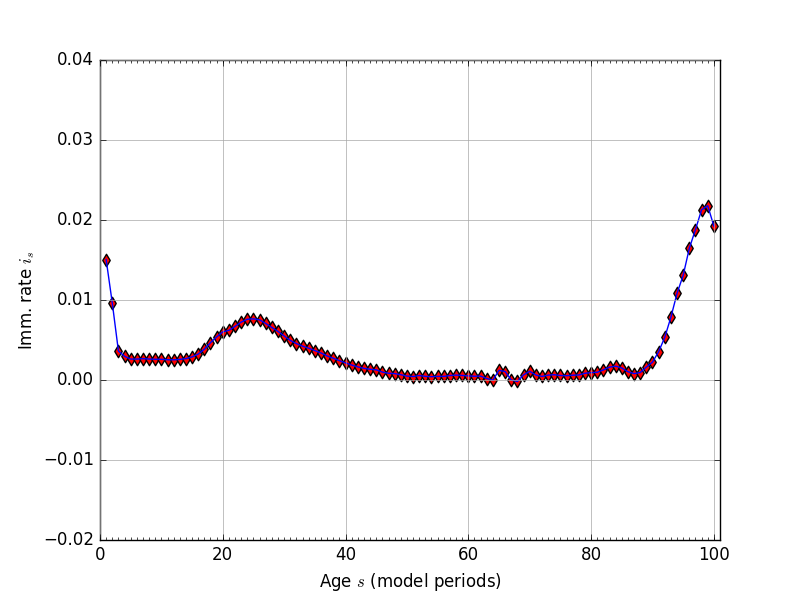
\includegraphics{./images/imm_rates_orig.png}}}
    \end{figure}

    We calculate our immigration rates for three different consecutive-year-periods of population distribution data (2010 through 2013). Our four years of population distribution by age data come from \citet{Census:2015}. The immigration rates $i_s$ that we use in our model are the residuals described in \eqref{EqPopImmRates} averaged across the three periods. Figure \ref{FigImmRates} shows the estimated immigration rates for $E+S=100$ and given the fertility rates from Section \ref{SecFert} and the mortality rates from Section \ref{SecMort}.

    In Section \ref{SecPopSSTP}, we describe a small adjustment that we make to the immigration rates after a certain number of periods in order to make computation of transition path equilibria of macroeconomic models compute more robustly.


  \subsection{Population steady-state and transition path}\label{SecPopSSTP}

    Macroeconomic models that use these demographic data often require information about mortality rates $\rho_{s,t}$ in order to solve for the households' optimization problems each period. They also often require the steady-state stationary population distribution $\bar{\omega}_{s}$ and population growth rate $\bar{g}_n$ as well as the full transition path of the stationary or normalized population distribution $\hat{\omega}_{s,t}$ and population growth rate $\tilde{g}_{n,t}$ from the current state to the steady-state. To solve for the steady-state and the transition path of the stationary population distribution, we write the stationary population dynamic equations \eqref{EqPopLawofmotionStat} and their matrix representation \eqref{EqPopLOMstatmat}.
    \begin{equation}\label{EqPopLawofmotionStat}
      \begin{split}
        \hat{\omega}_{1,t+1} &= \frac{(1-\rho_{0,t})\sum_{s=1}^{E+S}f_{s,t}\hat{\omega}_{s,t} + i_{1,t+1}\hat{\omega}_{1,t}}{1+\tilde{g}_{n,t+1}}\quad\forall t \\
        \hat{\omega}_{s+1,t+1} &= \frac{(1 - \rho_{s,t})\hat{\omega}_{s,t} + i_{s+1,t+1}\hat{\omega}_{s+1,t}}{1+\tilde{g}_{n,t+1}}\qquad\quad\:\forall t\quad\text{and}\quad 1\leq s \leq E+S-1
      \end{split}
    \end{equation}
    \begin{equation}\label{EqPopLOMstatmat}
      \begin{split}
        & \begin{bmatrix}
          \hat{\omega}_{1,t+1} \\ \hat{\omega}_{2,t+1} \\ \hat{\omega}_{2,t+1} \\ \vdots \\ \hat{\omega}_{E+S-1,t+1} \\ \hat{\omega}_{E+S,t+1}
        \end{bmatrix}= \frac{1}{1 + g_{n,t+1}} \times ... \\
        & \begin{bmatrix}
          (1-\rho_{0,t})f_{1,t}+i_{1,t+1} & (1-\rho_{0,t})f_{2,t} & (1-\rho_{0,t})f_{3,t} & \hdots & (1-\rho_{0,t})f_{E+S-1,t} & (1-\rho_{0,t})f_{E+S,t} \\
          1-\rho_{1,t} & i_{2,t+1} & 0 & \hdots & 0 & 0 \\
          0 & 1-\rho_{2,t} & i_{3,t+1} & \hdots & 0 & 0 \\
          \vdots & \vdots & \vdots & \ddots & \vdots & \vdots \\
          0 & 0 & 0 & \hdots & i_{E+S-1,t+1} & 0 \\
          0 & 0 & 0 & \hdots & 1-\rho_{E+S-1,t} & i_{E+S,t+1}
        \end{bmatrix}
        \begin{bmatrix}
          \hat{\omega}_{1,t} \\ \hat{\omega}_{2,t} \\ \hat{\omega}_{2,t} \\ \vdots \\ \hat{\omega}_{E+S-1,t} \\ \hat{\omega}_{E+S,t}
        \end{bmatrix}
      \end{split}
    \end{equation}

    We can write system \eqref{EqPopLOMstatmat} more simply in the following way. Note that the $\bm{\Omega}_t$ matrix has a $t$-subscript, signifying that the fertility, mortality, and immigration rates can be changing over time.
    \begin{equation}\label{EqPopLOMstatmat2}
      \bm{\hat{\omega}}_{t+1} = \frac{1}{1+g_{n,t+1}}\bm{\Omega}_t\bm{\hat{\omega}}_t \quad\forall t
    \end{equation}
    Assume that after some period $t\geq T_{end}$, all the fertility rates, mortality rates, and immigration rates reach a steady-state.
    \begin{equation}\label{EqFertMortImmSS}
      f_{s,t} = \bar{f}_s,\quad \rho_{s,t}=\bar{\rho}_s, \quad i_{s,t}=\bar{i}_s \quad\forall t\geq T_{end}
    \end{equation}
    Then for any $t\geq T_{end}$, we can specify a steady-state $\bm{\Omega}_t=\bm{\bar{\Omega}}$ matrix. The stationary steady-state population distribution $\bm{\bar{\omega}}$ is the eigenvector $\bm{\omega}$ with eigenvalue $(1+\bar{g}_n)$ of the matrix $\bm{\bar{\Omega}}$ that satisfies the following version of \eqref{EqPopLOMstatmat2}.
    \begin{equation}\label{EqPopLOMss}
      (1+\bar{g}_n)\bm{\bar{\omega}} = \bm{\bar{\Omega}}\bm{\bar{\omega}}
    \end{equation}

    \begin{proposition}
      If the age $s=1$ steady-state immigration rate is $\bar{i}_1>-(1-\bar{\rho}_0)\bar{f}_1$ and the other immigration rates are strictly positive $\bar{i}_s>0$ for all $s\geq 2$ such that all elements of $\bm{\bar{\Omega}}$ are nonnegative, then there exists a unique positive real eigenvector $\bm{\bar{\omega}}$ of the matrix $\bm{\bar{\Omega}}$, and it is a stable equilibrium.
    \end{proposition}

    \begin{proof}
      First, note that the matrix $\bm{\bar{\Omega}}$ is square and non-negative. This is enough for a general version of the Perron-Frobenius Theorem to state that a positive real eigenvector exists with a positive real eigenvalue. This is not yet enough for uniqueness. For it to be unique by a version of the Perron-Fobenius Theorem, we need to know that the matrix is irreducible. This can be easily shown. The matrix is of the form
      $$\bm{\bar{\Omega}} =
      \begin{bmatrix}
        * & *  & * & \hdots & * & * & *\\
        * & * & 0 & \hdots & 0 & 0 & 0 \\
        0 & * & * & \hdots & 0 & 0 & 0 \\
        \vdots & \vdots & \vdots & \ddots & \vdots & \vdots & \vdots \\
        0 & 0 & 0 & \hdots & *  & * & 0 \\
        0 & 0 & 0 & \hdots & 0 & * & *
      \end{bmatrix}
      $$
      Where each * is strictly positive. It is clear to see that taking powers of the matrix causes the sub-diagonal positive elements to be moved down a row and another row of positive entries is added at the top. None of these go to zero since the elements were all non-negative to begin with.
      $$\bm{\bar{\Omega}}^2 =
      \begin{bmatrix}
        * & *  & * & \hdots & * & * & *\\
        * & * & * & \hdots & * & * & * \\
        0 & * & * & \hdots & 0 & 0 & 0 \\
        \vdots & \vdots & \vdots & \ddots & \vdots & \vdots & \vdots \\
        0 & 0 & 0 & \hdots & *  & * & 0 \\
        0 & 0 & 0 & \hdots & 0 & * & *
      \end{bmatrix}; ~~~
      \bm{\bar{\Omega}}^{S+E-1} =
      \begin{bmatrix}
        * & *  & * & \hdots & * & * & *\\
        * & * & * & \hdots & * & * & * \\
        * & * & * & \hdots & * & * & * \\
        \vdots & \vdots & \vdots & \ddots & \vdots & \vdots & \vdots \\
        * & * & * & \hdots & *  & * & * \\
        0 & 0 & 0 & \hdots & 0 & * & *
      \end{bmatrix}
      $$
      $$\bm{\bar{\Omega}}^{S+E} =
      \begin{bmatrix}
        * & *  & * & \hdots & * & * & *\\
        * & * & * & \hdots & * & * & * \\
        * & * & * & \hdots & * & * & * \\
        \vdots & \vdots & \vdots & \ddots & \vdots & \vdots & \vdots \\
        * & * & * & \hdots & * & * & * \\
        * & * & * & \hdots & * & * & *
      \end{bmatrix}
      $$
      Existence of an $m \in \mathbb N $ such that $\left(\bf\bar{\Omega}^m\right)_{ij} \neq 0 ~~ ( > 0)$ is one of the definitions of an irreducible (primitive) matrix. It is equivalent to saying that the directed graph associated with the matrix is strongly connected. Now the Perron-Frobenius Theorem for irreducible matrices gives us that the equilibrium vector is unique.

      We also know from that theorem that the eigenvalue associated with the positive real eigenvector will be real and positive. This eigenvalue, $p$, is the Perron eigenvalue and it is the steady state population growth rate of the model. By the PF Theorem for irreducible matrices, $| \lambda_i | \leq p$ for all eigenvalues $\lambda_i$ and there will be exactly $h$ eigenvalues that are equal, where $h$ is the period of the matrix. Since our matrix $\bf\bar{\Omega}$ is aperiodic, the steady state growth rate is the unique largest eigenvalue in magnitude. This implies that almost all initial vectors will converge to this eigenvector under iteration.
    \end{proof}

    For a full treatment and proof of the Perron-Frobenius Theorem, see \citet{Suzumura:1983}. Because the population growth process is exogenous to the model, we calibrate it to annual age data for age years $s=1$ to $s=100$.

    Figure \ref{FigOrigVsFixSSpop} shows the steady-state population distribution $\bm{\bar{\omega}}$ and the population distribution after 120 periods $\bm{\hat{\omega}}_{120}$. Although the two distributions look very close to each other, they are not exactly the same.

    \begin{figure}[htbp]\centering \captionsetup{width=4.0in}
      \caption{\label{FigOrigVsFixSSpop}\textbf{Theoretical steady-state population distribution vs. population distribution at period $t=120$}}
      \fbox{\resizebox{4.0in}{3.0in}{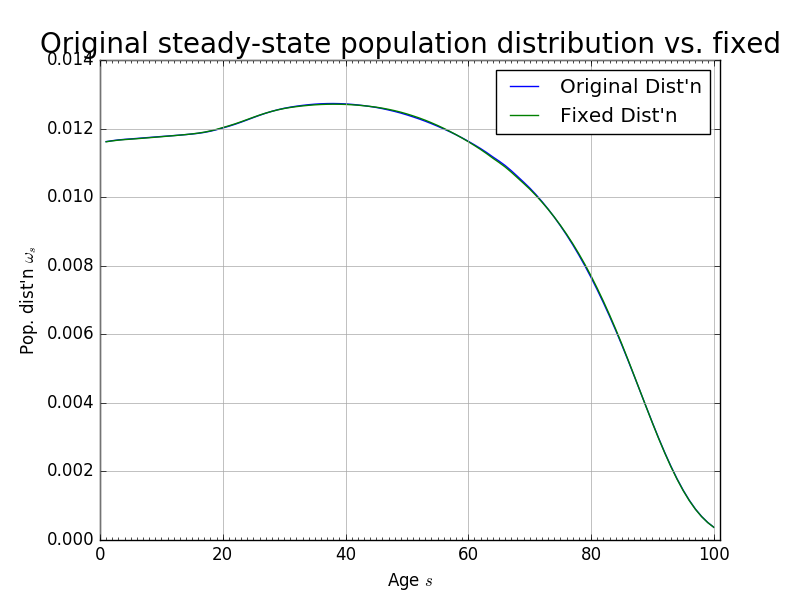
\includegraphics{./images/OrigVsFixSSpop.png}}}
    \end{figure}

    Further, we find that the maximum absolute difference between the population levels $\hat{\omega}_{s,t}$ and $\hat{\omega}_{s,t+1}$ was $1.3852\times 10^{-5}$ after 160 periods. That is to say, that after 160 periods, given the estimated mortality, fertility, and immigration rates, the population has not achieved its steady state. For convergence in our solution method over a reasonable time horizon, we want the population to reach a stationary distribution after $T_{end}$ periods. To do this, we artificially impose that the population distribution in period $T_{end}=120$ is the steady-state. As can be seen from Figure \ref{FigOrigVsFixSSpop}, this assumption is not very restrictive. Figure \ref{FigImmRateChg} shows the change in immigration rates that would make the period $t=120$ population distribution equal be the steady-state. The maximum absolute difference between any two corresponding immigration rates in Figure \ref{FigImmRateChg} is 0.0028.

    \begin{figure}[htbp]\centering \captionsetup{width=4.0in}
      \caption{\label{FigImmRateChg}\textbf{Original immigration rates vs. adjusted immigration rates to make fixed steady-state population distribution}}
      \fbox{\resizebox{4.0in}{3.0in}{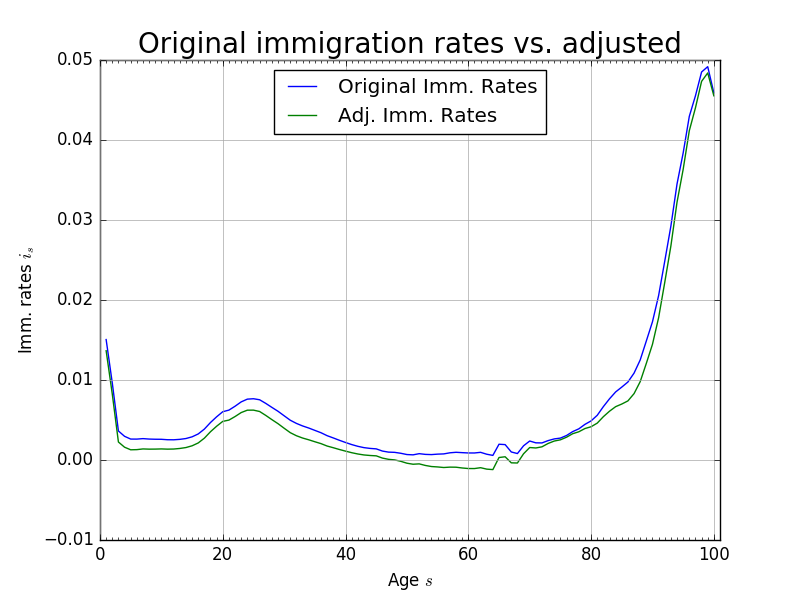
\includegraphics{./images/OrigVsAdjImm.png}}}
    \end{figure}

    The most recent year of population data come from \citet{Census:2015} population estimates for both sexes for 2013. We those data and use the population transition matrix \eqref{EqPopLOMstatmat2} to age it to the current model year of 2015. We then use \eqref{EqPopLOMstatmat2} to generate the transition path of the population distribution over the time period of the model. Figure \ref{FigPopDistPath} shows the progression from the 2013 population data to the fixed steady-state at period $T_{end}=120$. The time path of the growth rate of the economically active population $\tilde{g}_{n,t}$ is shown in Figure \ref{FigGrowthPath}.

    \begin{figure}[htbp]\centering \captionsetup{width=4.0in}
      \caption{\label{FigPopDistPath}\textbf{Stationary population distribution at periods along transition path}}
      \fbox{\resizebox{4.0in}{3.0in}{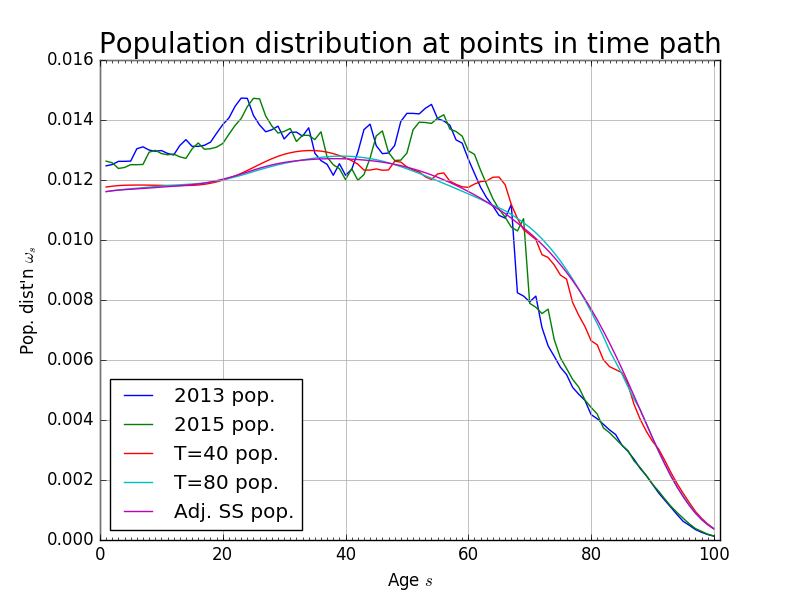
\includegraphics{./images/PopDistPath.png}}}
    \end{figure}

    \begin{figure}[htbp]\centering \captionsetup{width=4.0in}
      \caption{\label{FigGrowthPath}\textbf{Time path of the population growth rate $\tilde{g}_{n,t}$}}
      \fbox{\resizebox{4.0in}{3.0in}{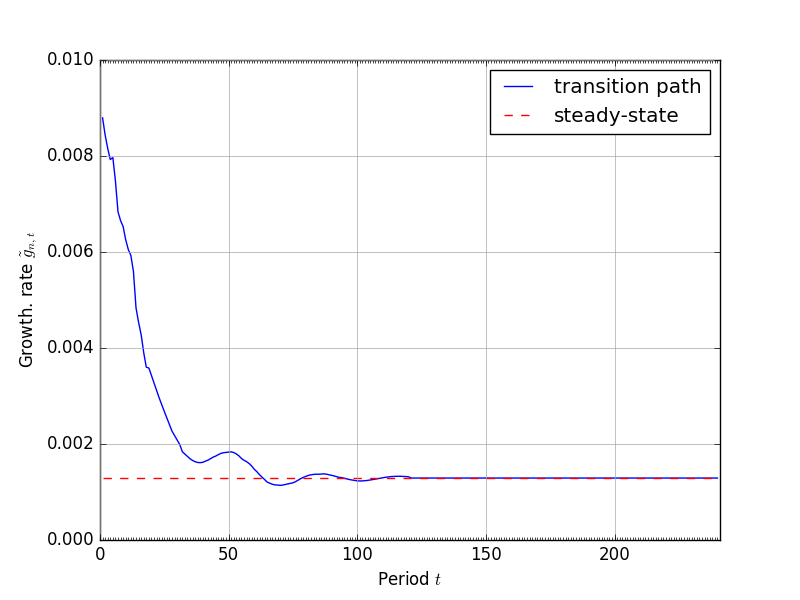
\includegraphics{./images/GrowthPath.png}}}
    \end{figure}


\section{Interpolation and Curve Fitting}\label{SecInterpCurvFit}

  Interpolation is a general term than signifies, in its broadest sense, the prediction of variable value

  \subsection{Interpolation}\label{SecInterp}

    Interpolation


  \subsection{Curve fitting}\label{SecCurvFit}

    Two important functions that we use in curve fitting in this project are a parameterized arctangent and a parameterized exponential. For data that monotonically increase or decrease in both value and slope from or to some horizontal asymptote, the three-parameter negative exponential is a flexible and parsimonious function.
    \begin{equation}\label{EqExp3param}
      (EX_3):\quad f(x|a,b,c) = e^{ax^2 + bx + c} \quad\forall x, a, b, c
    \end{equation}
    For monotonic data that start out with low slope, then increase in slope, then decrease again in slope, the parameterized arctangent function is a flexible and parsimonious function.
    \begin{equation}\label{EqArctan3param}
      (Arctan_3):\quad f(x|a,b,c) = \arctan\left(ax + b\right) + c \quad\forall x, a, b, c
    \end{equation}


\section{Estimation with Hierarchical Distribution Families}\label{SecDistFam}

  It is often valuable to fit curves or distributions with parametric functions. These functions use a limited and fixed number of parameters to capture general shapes of different families of curves. One such class of univariate probability density functions with positive support $x\geq 0$ is the generalized beta family of distributions shown in Figure \ref{FigGBtree} taken from \citet[Fig. 2]{McDonaldXu:1995}.

  \begin{figure}[htb]\centering\captionsetup{width=6.0in}
    \caption{\textbf{Generalized beta family of distributions (McDonald and Xu, Fig. 2, 1995)}}\label{FigGBtree}
    \fbox{\resizebox{6.0in}{4.0in}{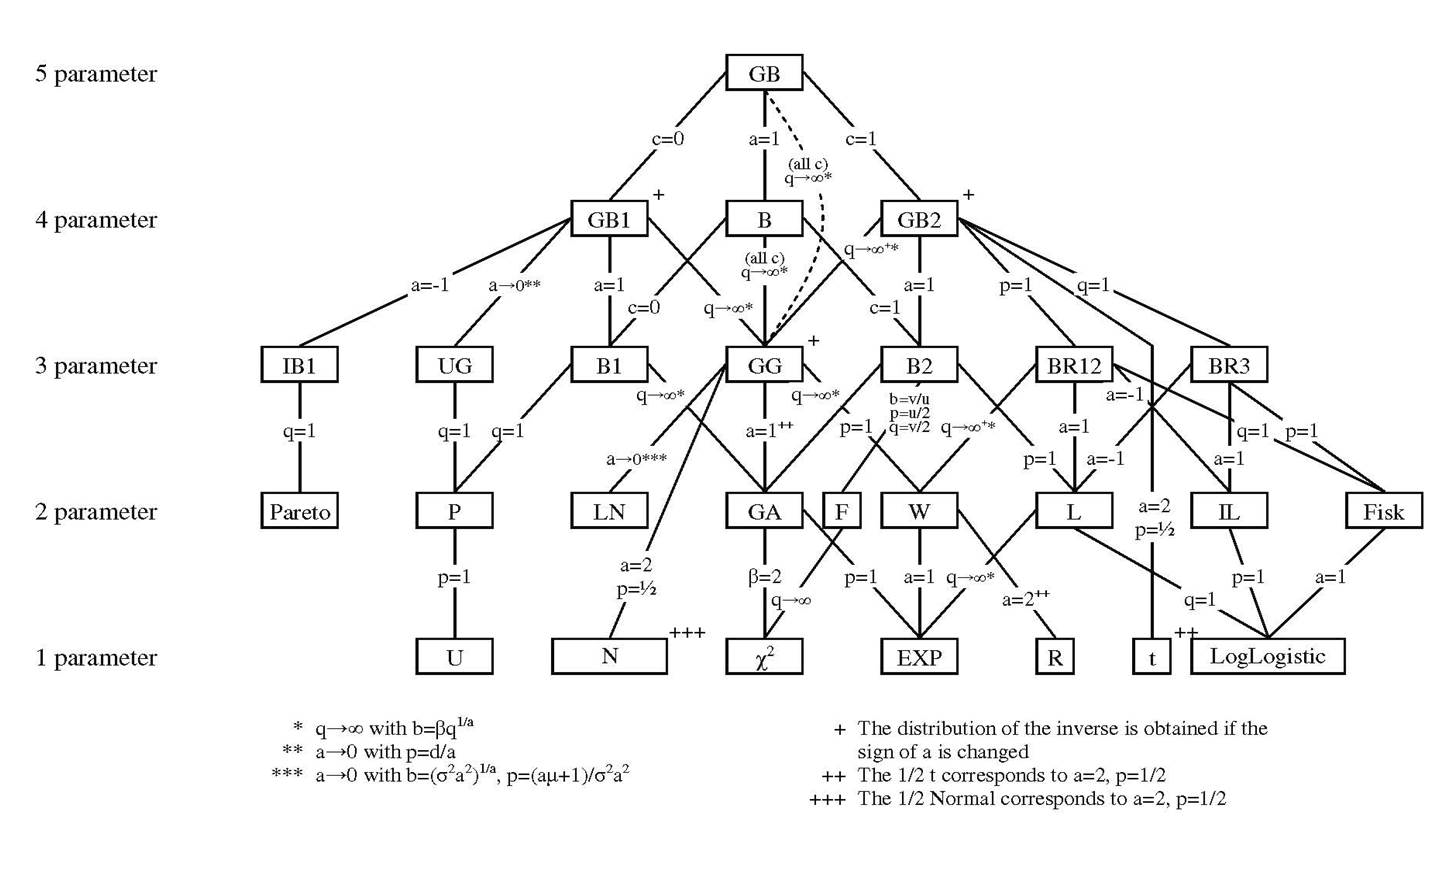
\includegraphics{images/GBtree.png}}}
  \end{figure}

  Two of the distributions from Figure \ref{FigGBtree} that we will use for curve fitting are the two-parameter gamma $GA(\alpha,\beta)$ distribution defined in \eqref{EqGAdist} and its three-parameter parent distribution the generalized gamma $GG(\alpha,\beta,m)$ defined in \eqref{EqGGdist}.\footnote{Code for the probability density functions of the $GA$ distribution and $GG$ distribution can be found in the \href{https://github.com/OpenSourceEcon/DynamicPop/blob/master/code/distributions.py}{\texttt{distributions.py}} module as the \texttt{GA\_pdf()} and \texttt{GG\_pdf()} functions, respectively.}
  \begin{equation}\label{EqGAdist}
    \begin{split}
      \text(GA):\quad f(x|\alpha,\beta) &= \frac{1}{\beta^\alpha \Gamma(\alpha)}x^{\alpha-1}e^{-\frac{x}{\beta}}, \quad x\in[0,\infty],\:\alpha,\beta>0 \\
      &\text{where}\quad \Gamma(z)\equiv \int_0^\infty v^{z-1}e^{-v}dv
    \end{split}
  \end{equation}
  \begin{equation}\label{EqGGdist}
    \begin{split}
      \text{(GG)}:\quad f(x|\alpha,\beta,m) &= \frac{m}{\beta^\alpha \Gamma\left(\frac{\alpha}{m}\right)}x^{\alpha-1}e^{-\left(\frac{x}{\beta}\right)^m}, \quad x\in[0,\infty],\:\alpha,\beta,m>0 \\
      &\text{where}\quad \Gamma(z)\equiv \int_0^\infty v^{z-1}e^{-v}dv
    \end{split}
  \end{equation}


\section{Exercises}\label{SecExercises}

  \renewcommand\theenumi{\alph{enumi}}

  \begin{exercise}\label{ExFertEst}
    Define the fertility rate as $f_{s,t}$ which signifies the percent of age-$s$ individuals that have children in year $t$. This fertility rate must account for both male and female population.
    \begin{enumerate}
      \item Get U.S. fertility rate data by age for as many years as possible from 1980 to the most recent year available. If the data for a given year $t$ are less detailed than fertility rate for every age year, interpolate every age year using a cubic spline. If the data do not cover from age 21 up to age 100, choose a method to extrapolate the end points such that the extrapolation function has the same value and slope as the interpolated function at the interpolated function end points and that the function has monotonic slope and finishes at a logical endpoint. Good extrapolation function candidates are the three-parameter exponential \eqref{EqExp3param} or the three-parameter arctangent \eqref{EqArctan3param} functions.
      \item For each year of fertility-rate-by-age data $f_{s,t}$, fit a four-parameter function to the data by GMM (minimize the sum of squared errors), which function is comprised of the three-parameter generalized gamma $GG(\alpha,\beta,m)$ distribution defined in \eqref{EqGGdist} and scaled by parameter $\chi>0$.\footnote{This new function is only a probability density function for $\chi=1$.}
      \begin{equation}\label{EqFert4param}
        \begin{split}
          g(f_{s,t}|\chi_t,\alpha_t,\beta_t,m_t) &= \chi_t\frac{m_t}{\beta_t^{\alpha_t} \Gamma\left(\frac{\alpha_t}{m_t}\right)}f_{s,t}^{\alpha_t-1}e^{-\left(\frac{f_{s,t}}{\beta_t}\right)^{m_t}}, \quad\forall t,\: f_{s,t}\in[0,\infty],\:\chi_t,\alpha_t,\beta_t,m_t>0 \\
          &\text{where}\quad \Gamma(z)\equiv \int_0^\infty v^{z-1}e^{-v}dv
        \end{split}
      \end{equation}
      Plot the estimated fertility rate functions $g(f_{s,t}|\hat{\chi}_t,\hat{\alpha}_t,\hat{\beta}_t,\hat{m}_t)$ for each year of the data. Make separate time series plots for each of the four estimated parameters $\hat{\chi}_t$, $\hat{\alpha}_t$, $\hat{\beta}_t$, $\hat{m}_t$.
      \item Using least squares, fit a negative arctangent \eqref{EqArctan3param} or exponential function \eqref{EqExp3param} to each of the four estimated parameters time series. If the current period is $t=2020$, make sure that the fitted functions asymptote to a clear value around period $t=2100$. Plot each of the four fitted functions against the respective data for periods $1980\leq t\leq 2100$.
      \item Using your four fitted functions for the time path of parameters of the $GG$ function $\hat{\chi}_t$, $\hat{\alpha}_t$, $\hat{\beta}_t$, $\hat{m}_t$, plot for each year $1980\leq t\leq 2100$ the estimated fertility rate by age $f_{s,t}$.
    \end{enumerate}
  \end{exercise}

  \begin{exercise}\label{ExMortEst}
    Define the mortality rate as $\rho_{s,t}$ which signifies the percent of age-$s$ individuals that die in period $t$ (i.e., do not live to period $t+1$).
    \begin{enumerate}
      \item Get U.S. mortality rate data by age for as many years as possible from 1980 to the most recent year available. If the data for a given year $t$ are less detailed than mortality rate for every age year, interpolate every age year using a cubic spline. Force the mortality rate at age 100 to be 1.0 (or 100\%). If the data do not cover from age 21 up, choose a method to extrapolate the end points such that the extrapolation function has the same value and slope as the interpolated function at the interpolated function end points and that the function has monotonic slope and finishes at a logical endpoint. Good extrapolation function candidates are the three-parameter exponential \eqref{EqExp3param} or the three-parameter arctangent \eqref{EqArctan3param} functions.
      \item For each year of mortality-rate-by-age data $\rho_{s,t}$, fit a three-parameter exponential function \eqref{EqExp3param} to the data by GMM (minimize the sum of squared errors).
      \begin{equation}\label{EqMort3param}
        g(\rho_{s,t}|a_t,b_t,c_t) = e^{a_t(\rho_{s,t})^2 + b_t\rho_{s,t} + c_t}, \quad\forall t,a,b,c,\quad \rho_{s,t}\in[0,1]
      \end{equation}
      Plot the estimated mortality rate functions $g(\rho_{s,t}|\hat{a}_t,\hat{b}_t,\hat{c}_t)$ for each year of the data. Make separate time series plots for each of the three estimated parameters $\hat{a}_t$, $\hat{b}_t$, $\hat{c}_t$.
      \item Using least squares, fit a negative arctangent \eqref{EqArctan3param} or exponential function \eqref{EqExp3param} to each of the three estimated parameters time series. If the current period is $t=2020$, make sure that the fitted functions asymptote to a clear value around period $t=2100$. Plot each of the three fitted functions against the respective data for periods $1980\leq t\leq 2100$.
      \item Using your three fitted functions for the time path of parameters of the three-parameter exponential $EX_3$ function $\hat{a}_t$, $\hat{b}_t$, $\hat{c}_t$, plot for each year $1980\leq t\leq 2100$ the estimated mortality rate by age $\rho_{s,t}$.
    \end{enumerate}
  \end{exercise}

  \begin{exercise}\label{ExImmEst}
    Define the normalized population $\hat{\omega}_{s,t}$ as the percent of the population in period $t$ that is age $s$, such that $\sum_{s=1}^S\tilde{\omega}_{s,t} = 1$ for all $t$. Define the immigration rate $i_{s,t}$ as the number of age-$s$ immigrants in the current period as a percent of the age-$s$ population in the previous period (i.e., the number of immigrants in the current period equals $i_{s,t}\omega_{s,t-1}$).
    \begin{enumerate}
      \item Solve for the immigration rate of each year of past data $\{i_{s,t}\}_{s=1,t=1981}^{E+S,t=2019}$ using population data, fertility rates, and mortality rates using equations \eqref{EqPopImmRates}.
      \item Fit some parametric functional form to each year of immigration data.
      \item Find the asymptote of the parameters by period $T_{end}=2100$.
    \end{enumerate}
  \end{exercise}

  \begin{exercise}\label{ExImmEst}
    Use your estimated time paths of the fertility rates, mortality rates, and immigration rates, and their respective steady-state distributions for periods $t\geq T_{end}=2100$ to solve for the transition path of the population distribution $\omega_{s,t}$ from its current state $\omega_{s,t=2020}$ to the steady state at $t=2100$.
  \end{exercise}



  \renewcommand\theenumi{\roman{enumi}}


\bibliography{demog.bib}


\end{document}
